\section{Interval Models}

An interval is modeled in such a way that enables a quantitative comparison of intervals to one another for similarity. The models that we use to detect SFG phases includes the instruction working set, basic block vectors, and Intel Top-Down. 

\subsection{Instruction Working Set Signature}

An instruction working set (IWS)~\cite{Dhodapkar:2002:MMH} is the set of instructions touched over a fixed interval of time. The relative working set distance between intervals $i$ and $i-1$ is defined as 

\begin{center}
$\delta_{i,i-1} = \frac{||W_i \bigcup W_{i-1}||-||W_i \bigcap W_{i-1}||}{||W_i \bigcup W_{i-1}||}$
\end{center}
where $W_i$ is the working set for interval $i$.
 
A working set signature is a lossy-compressed representation of a working set. The program counter is sampled over a fixed interval of instructions. A hashing function is applied to the sample to set a bit in an $n$-bit vector, which represents the signature (See Figure~\ref{fig:signature}). Phase changes are detected by computing the relative signature distance between intervals and comparing the distance against some pre-determined threshold. The hardware complexity of this technique is dependent on the working set size.

\begin{figure}[htbp]
  \begin{center}
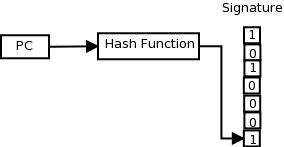
\includegraphics[width=0.60\columnwidth]{figs/workingsetsignature}
  \end{center}
  \caption{Generating the working set signature.}
  \label{fig:signature}
\end{figure}

\subsection{Basic Block Vectors}

Basic block vectors (BBV)~\cite{Sherwood:2003:DEP} encodes the execution frequency of basic blocks over an interval. BBVs can be approximated using an array of accumulators (counters) that tracks the number of instructions executed by a basic block in a given execution interval (see Figure~\ref{fig:bbv}). When a branch PC is encountered, a hash function is applied to the PC to determine an index into the accumulator table in order to increment the appropriate counter by the number of committed instructions since the last branch instruction. The BBV difference between intervals is computed using the manhattan distance. A phase change is determined by comparing the BBV difference to a difference threshold. The hardware required to implement BBVs includes an N-bit wide RAM array for the accumulator table, sampling hardware to detect branch instructions and analyze the retire stream, and an N-bit adder to update the accumulator table. The hardware complexity of BBV is much higher compared to working set signatures. 

\begin{figure}[htbp]
  \begin{center}
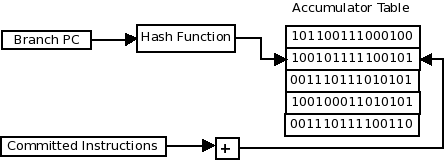
\includegraphics[width=0.80\columnwidth]{figs/bbv}
  \end{center}
  \caption{BBV accumulator table update technique.}
  \label{fig:bbv}
\end{figure}

\subsection{Intel Top-Down Classification}
\label{sec:topdown}

Intel Top-Down (ITD)~\cite{Yasin:2014:TDM} classifies pipeline activity very broadly into four categories: \textbf{frontend bound}, \textbf{bad speculation}, \textbf{retiring}, and \textbf{backend bound} (see Figure~\ref{fig:topdown2}). Each of these categories can be broken down even further and differently depending on the architecture. Below we describe the four top-level categories for the LEON3 (32-bit SPARC V8 architecture) instruction pipeline since this is the architecture used in our measurements.

\textbf{Frontend Bound.} The frontend includes the front portion of the pipeline where the branch predictor predicts the next address, instructions are fetched and decoded, and the register file is accessed. The frontend prepares instructions to be executed by the backend of the processor. Cycles are classified as frontend bound when the frontend undersupplies the backend of the pipeline (e.g. instruction cache misses).

\textbf{Bad speculation.} This category captures inefficiency in the pipeline due to incorrect speculation by the branch predictor. This includes issued instructions that do not eventually get retired. These instructions are annulled (i.e. has no effect and effectively not executed) in the LEON3.  

\textbf{Retiring.} This category is for issued instructions that eventually get retired. 

\textbf{Backend Bound.} A cycle is classified as backend bound when a new instruction is not issued to the execution unit in a given cycle while the frontend of the pipeline is not stalled. This may be due to data cache misses or overloaded functional units. The backend category can be further broken down into \emph{core bound} and \emph{memory bound}. 

\begin{itemize}
\item [--] \underline{Core bound} includes stalls due to overloaded functional units.
\item [--] \underline{Memory bound} includes store bound (i.e. high number of buffered stores), L1 bound (cache access), and memory bound (cache miss).
\end{itemize}

\begin{figure}[htbp]
  \begin{center}
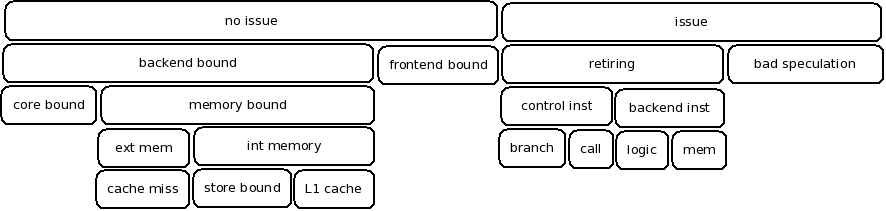
\includegraphics[width=0.99\columnwidth]{figs/topdown2}
  \end{center}
  \caption{An example of the Intel Top-Down processor activity categories.}
  \label{fig:topdown2}
\end{figure}

Traditionally, the ITD categories has been used for the purpose of detecting sources of performance bottlenecks. The motivation for using the ITD classification to detect SFG phases is that the different categories provides different levels of detail regarding pipeline activity, which we think is a good model for program behavior. Furthermore, hardware complexity is significantly reduced since only a finite vector of size $n$ is necessary to store the frequency of each category over an interval, where $n$ is the number of categories at each level. By comparison, the hardware complexity is a function of the number of unique instructions in the case of IWS and the number of unique basic blocks in the case of BBVs, which can be difficult to determine a priori. The ITD vector difference between intervals is computed using the Manhattan distance, similar to the BBV difference.




